\section{Các thuật toán tìm kiếm không có thông tin: BFS, DFS, IDS}

Ba thuật toán trong mục này không dùng heuristic ước lượng khoảng cách đến đích, và đều coi mỗi nước đi có chi phí 1. Đề cho phép dùng IDS thay cho DFS; nhóm cài đặt \textbf{cả hai} và đưa cả hai vào thực nghiệm. Cả ba được cài đặt bằng tay, chỉ dùng các cấu trúc dữ liệu chuẩn của Python (\texttt{collections.deque}, \texttt{list}, \texttt{dict}, \texttt{set}).

\subsection{Khung tìm kiếm trên đồ thị dùng chung}

Ba thuật toán cùng một khung; chúng chỉ khác nhau ở \textbf{cấu trúc dữ liệu của frontier} (tập các nút đã sinh nhưng chưa mở rộng) và \textbf{cách chọn nút để mở rộng tiếp theo}:

\begin{Verbatim}[breaklines=true, fontsize=\footnotesize, frame=single]
GRAPH-SEARCH(problem):
    frontier <- { s0 }                  # s0 = problem.initial_state
    reached  <- { s0 }                  # các trạng thái đã gặp, kèm con trỏ cha
    trong khi frontier không rỗng:
        s <- CHỌN-VÀ-LẤY-RA(frontier)   # điểm khác nhau giữa các thuật toán
        nếu s là đích: dựng lại đường đi bằng cách lần ngược theo con trỏ cha
        mở rộng s: với mỗi (a, s') trong successors(s):
            nếu s' chưa có trong reached:
                ghi nhận s' (cha = s, hành động = a), đưa s' vào frontier
    trả về thất bại
\end{Verbatim}

Khung trên kiểm tra đích lúc lấy nút ra, nên nút đích không bao giờ bị mở rộng. DFS và IDS dùng đúng cách này; BFS kiểm tra sớm hơn, ngay khi nút được sinh ra (mục 4.2.3).

{\renewcommand{\arraystretch}{1.25}
\begin{longtable}{|>{\raggedright\arraybackslash}p{0.083\linewidth}|>{\raggedright\arraybackslash}p{0.306\linewidth}|>{\raggedright\arraybackslash}p{0.182\linewidth}|>{\raggedright\arraybackslash}p{0.289\linewidth}|}
\hline
\textbf{Thuật toán} & \textbf{Frontier} & \textbf{Chọn nút} & \textbf{Ý nghĩa} \\ \hline
\endhead
\hline
\endlastfoot
BFS & Hàng đợi FIFO (\texttt{deque}) & Nút vào sớm nhất & Duyệt theo từng lớp độ sâu \\ \hline
DFS & Ngăn xếp LIFO (\texttt{list}) & Nút vào muộn nhất & Đi sâu trước, quay lui sau \\ \hline
IDS & Ngăn xếp, có giới hạn độ sâu tăng dần & Như DFS trong mỗi lượt & Lặp lại DFS với giới hạn 1, 2, 3, … \\
\end{longtable}
}

\textbf{Ghi nhận đường đi.} Thay vì lưu kèm danh sách hành động trong mỗi phần tử của frontier (tốn thêm bộ nhớ tỉ lệ với độ sâu cho mỗi nút), mỗi trạng thái chỉ lưu \texttt{(trạng thái cha, hành động đã dùng)} trong từ điển \texttt{parent}. Khi tìm thấy đích, đường đi được dựng bằng cách lần ngược từ đích về trạng thái đầu rồi đảo thứ tự.

\textbf{Quy ước đếm số nút mở rộng (expanded nodes).} Một nút được tính là \emph{đã mở rộng} khi nó được lấy ra khỏi frontier \textbf{và} các nút con của nó được sinh ra (gọi \texttt{successors}). Nút đích không được tính vì không cần sinh nút con của nó. Quy ước này được áp dụng thống nhất cho mọi thuật toán thông qua \texttt{MetricsTracker.count\_\allowbreak{}expansion()}, nhờ vậy các con số có thể so sánh với nhau. Với IDS, số này là tổng cộng dồn qua tất cả các lượt lặp.

\subsection{Tìm kiếm theo chiều rộng (BFS)}

\subsubsection{Ý tưởng}

BFS mở rộng toàn bộ các trạng thái cách trạng thái đầu 0 nước đi, rồi đến 1 nước, 2 nước, … Mọi trạng thái ở độ sâu k đều được mở rộng trước mọi trạng thái ở độ sâu k+1. Frontier là hàng đợi FIFO, cài đặt bằng \texttt{collections.deque} để cả \texttt{append} (thêm vào cuối) lẫn \texttt{popleft} (lấy từ đầu) đều có chi phí O(1).

\subsubsection{Mã giả}

\begin{Verbatim}[breaklines=true, fontsize=\footnotesize, frame=single]
BFS(problem):
    s0 <- problem.initial_state
    nếu is_goal(s0): trả về []                       # 0 nước đi, 0 nút mở rộng
    frontier <- deque([s0])
    parent   <- { s0: None }                           # đồng thời là tập các trạng thái đã thăm
    trong khi frontier không rỗng:
        s <- frontier.popleft()
        expanded <- expanded + 1
        với mỗi (a, s') trong successors(s):          # thứ tự U, D, L, R (S nếu đang tách)
            nếu s' chưa có trong parent:
                parent[s'] <- (s, a)
                nếu is_goal(s'): trả về reconstruct(parent, s')   # kiểm tra đích sớm
                frontier.append(s')
    trả về None
\end{Verbatim}

\subsubsection{Các quyết định cài đặt}

\begin{itemize}
\item \textbf{Kiểm tra đích sớm.} Đích được kiểm tra ngay khi trạng thái được \emph{sinh ra}, không đợi đến khi nó được lấy khỏi hàng đợi. Điều này đúng vì mọi nước đi có cùng chi phí nên trạng thái đích được sinh ra đầu tiên chắc chắn nằm ở độ sâu nhỏ nhất. Cách làm này tránh việc phải mở rộng thêm cả một lớp độ sâu trước khi trả về (Russell và Norvig, AIMA). Hệ quả là nút đích ở độ sâu d được phát hiện khi mở rộng một nút ở độ sâu d−1, và Hình 2 cho thấy lớp cuối cùng được mở rộng chỉ có độ sâu d−1.
\item \textbf{Từ điển \texttt{parent} đóng hai vai trò}: lưu con trỏ cha để dựng đường đi và là tập đã thăm để chống lặp. Một trạng thái chỉ vào frontier khi chưa từng xuất hiện trong \texttt{parent}, do đó mỗi trạng thái được mở rộng tối đa một lần.
\item \textbf{Frontier chỉ chứa trạng thái}, không chứa đường đi, như đã nêu ở mục 4.1.
\end{itemize}

\subsubsection{Ví dụ chạy tay trên màn g1\_basic\_01}

Màn gồm lưới 3 hàng × 6 cột toàn sàn thường, xuất phát tại (0,0), đích tại (2,5). Kí hiệu trạng thái: chữ cái là tư thế (S: đứng, H: nằm ngang, V: nằm dọc) kèm ô neo (hàng, cột).

{\renewcommand{\arraystretch}{1.25}
\begin{longtable}{|>{\raggedleft\arraybackslash}p{0.073\linewidth}|>{\raggedright\arraybackslash}p{0.122\linewidth}|>{\raggedright\arraybackslash}p{0.349\linewidth}|>{\raggedright\arraybackslash}p{0.316\linewidth}|}
\hline
\textbf{Bước} & \textbf{Nút được lấy ra} & \textbf{Các nút con sinh ra (hành động: trạng thái)} & \textbf{Ghi chú} \\ \hline
\endhead
\hline
\endlastfoot
1 & S(0,0) & D: V(1,0); R: H(0,1) & U và L ra ngoài lưới nên bị loại \\ \hline
2 & V(1,0) & U: S(0,0); R: V(1,1) & S(0,0) đã có trong \texttt{parent} nên bị bỏ qua \\ \hline
3 & H(0,1) & D: H(1,1); L: S(0,0); R: S(0,3) & S(0,0) bị bỏ qua \\ \hline
4 & V(1,1) & U: S(0,1); L: V(1,0); R: V(1,2) & V(1,0) bị bỏ qua \\
\end{longtable}
}

Số nút được mở rộng theo từng độ sâu là \texttt{[1, 2, 3, 7, 6, 8, 9, 5]} (tổng 41 nút). Nút đích được sinh ra ở độ sâu 8 khi đang mở rộng một nút ở độ sâu 7, và đường đi trả về là \textbf{DRRURDDR} (8 nước đi).

\subsubsection{Tính chất và chứng minh}

\textbf{Tính dừng và tính đầy đủ.} Không gian trạng thái hữu hạn (mục 3.2) và mỗi trạng thái vào frontier tối đa một lần, nên vòng lặp luôn kết thúc. Nếu đích đạt tới được thì nó sẽ được sinh ra ở một lúc nào đó, vì mọi trạng thái đạt tới được đều lần lượt được mở rộng. Nếu frontier cạn mà chưa gặp đích, màn không có lời giải. Do đó BFS đầy đủ và quyết định được tính giải được của màn.

\textbf{Tính tối ưu theo số nước đi.} Chứng minh bằng quy nạp theo độ sâu k: \emph{mọi trạng thái ở độ sâu k (khoảng cách ngắn nhất tính bằng số nước đi từ trạng thái đầu) được đưa vào hàng đợi trước mọi trạng thái ở độ sâu k+1, và \texttt{parent} của nó lưu đúng một đường đi có độ dài k.}

\begin{itemize}
\item Cơ sở: độ sâu 0 chỉ có s0.
\item Bước quy nạp: mọi trạng thái ở độ sâu k+1 có một nút cha ở độ sâu k. Theo giả thiết, các nút ở độ sâu k đều được lấy ra (và mở rộng) trước các nút ở độ sâu k+1, nên trạng thái ở độ sâu k+1 được sinh ra đầu tiên từ một nút độ sâu k. Không nút nào ở độ sâu lớn hơn có thể sinh ra nó sớm hơn vì chúng được lấy ra sau.
\end{itemize}

Do đó lần đầu một trạng thái được phát hiện chính là lúc nó được phát hiện bằng đường ngắn nhất, và đích được phát hiện lần đầu cho lời giải có số nước đi nhỏ nhất. Tính chất này chỉ đảm bảo tối ưu theo \textbf{số nước đi}; không đảm bảo tối ưu theo \texttt{physics\_\allowbreak{}cost} (mục 6.5).

\textbf{Độ phức tạp.} Mỗi trạng thái được mở rộng tối đa một lần, mỗi lần sinh tối đa b nút con (b ≤ 4, hoặc 5 khi đang tách) và mỗi thao tác tra bảng băm là O(1). Thời gian là O(b·\textbar{}S\textbar{}) = O(\textbar{}S\textbar{}), và theo độ sâu lời giải d còn bị chặn bởi O(b$^{d}$). Bộ nhớ là O(\textbar{}S\textbar{}) vì phải giữ cả frontier lẫn \texttt{parent}. Thực tế số nút theo từng độ sâu tăng chậm hơn nhiều so với b$^{d}$ vì đồ thị trạng thái có nhiều đường song song và chu trình (Hình 2).

\begin{figure}[!htbp]
\centering
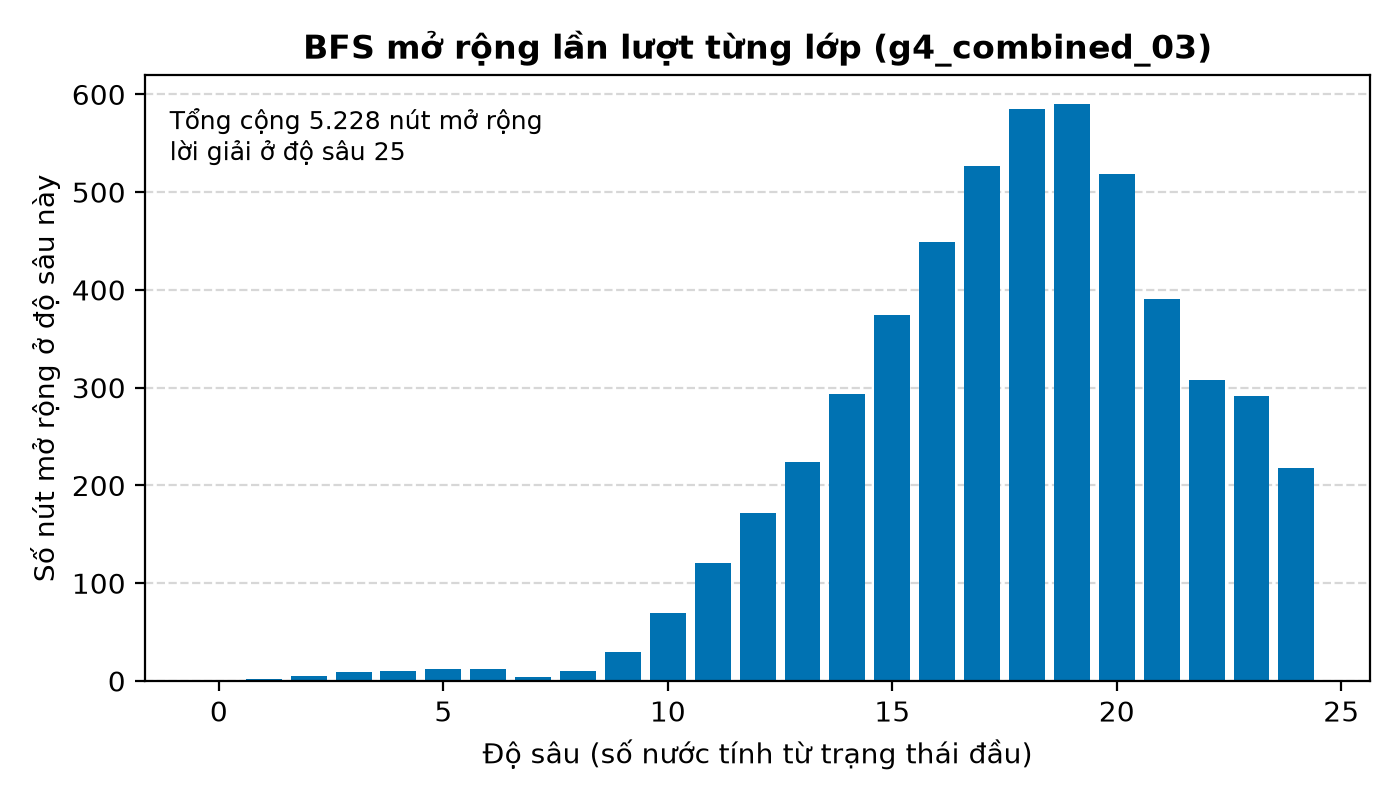
\includegraphics[width=\linewidth,height=0.45\textheight,keepaspectratio]{images/fig_bfs_layers.png}
\caption{Số nút BFS mở rộng ở từng độ sâu trên màn g4\_combined\_03: tổng 5.228 nút, lời giải ở độ sâu 25. Số nút theo lớp tăng đến cực đại ở độ sâu 18–19 rồi giảm.}
\end{figure}

\subsection{Tìm kiếm theo chiều sâu (DFS)}

\subsubsection{Ý tưởng}

DFS luôn đi sâu theo một nhánh cho đến khi gặp ngõ cụt (mọi nước đi đều dẫn đến trạng thái đã thăm hoặc không hợp lệ), rồi quay lui để thử nhánh khác. Frontier là ngăn xếp LIFO. Thuật toán được cài đặt \textbf{bằng ngăn xếp tường minh} (một \texttt{list} với \texttt{append} và \texttt{pop}) mà không dùng đệ quy, để không gặp \texttt{RecursionError} khi lời giải dài (DFS tìm được lời giải 304 nước ở màn g4\_combined\_02).

\subsubsection{Mã giả}

\begin{Verbatim}[breaklines=true, fontsize=\footnotesize, frame=single]
DFS(problem, max_depth = None):
    s0 <- problem.initial_state
    nếu is_goal(s0): trả về []
    stack   <- [(s0, 0)]
    parent  <- { s0: None };  visited <- { s0 }
    trong khi stack không rỗng:
        (s, depth) <- stack.pop()
        nếu is_goal(s): trả về reconstruct(parent, s)
        nếu max_depth != None và depth >= max_depth: tiếp tục vòng lặp       # cắt nhánh
        expanded <- expanded + 1
        với mỗi (a, s') trong reversed(successors(s)):
            nếu s' chưa có trong visited:
                visited.add(s');  parent[s'] <- (s, a)
                stack.append((s', depth + 1))
    trả về None
\end{Verbatim}

\subsubsection{Các quyết định cài đặt}

\begin{itemize}
\item \textbf{Duyệt \texttt{reversed(successors(s))}.} Ngăn xếp lấy phần tử \emph{đưa vào sau cùng} ra trước. Đưa các nút con vào theo thứ tự ngược lại thì nút con \emph{đầu tiên} theo thứ tự quy ước (Lên) nằm ở đỉnh và được duyệt trước, nhờ đó thứ tự duyệt vẫn là U, D, L, R. Nếu bỏ \texttt{reversed}, DFS sẽ duyệt Phải trước và cho một lời giải khác.
\item \textbf{Đánh dấu đã thăm lúc đưa vào ngăn xếp} (không phải lúc lấy ra). Mỗi trạng thái vào ngăn xếp tối đa một lần nên ngăn xếp không chứa bản sao.
\item \textbf{Kiểm tra đích lúc lấy ra khỏi ngăn xếp.} Khác với BFS, đích đầu tiên mà DFS gặp không nhất thiết ở độ sâu nhỏ nhất, nên kiểm tra sớm không mang lại lợi ích về tính tối ưu. Nút đích được kiểm tra trước khi tính vào \texttt{expanded}, do đó không bị đếm, nhất quán với BFS.
\item \textbf{Tham số \texttt{max\_\allowbreak{}depth}} là giới hạn độ sâu tùy chọn; cơ chế cắt nhánh này là nền tảng của IDS.
\end{itemize}

\subsubsection{Ví dụ chạy tay trên màn g1\_basic\_01}

Ngăn xếp được viết với đỉnh ở bên phải.

{\renewcommand{\arraystretch}{1.25}
\begin{longtable}{|>{\raggedleft\arraybackslash}p{0.085\linewidth}|>{\raggedright\arraybackslash}p{0.161\linewidth}|>{\raggedright\arraybackslash}p{0.406\linewidth}|>{\raggedright\arraybackslash}p{0.208\linewidth}|}
\hline
\textbf{Bước} & \textbf{Nút lấy ra (đỉnh)} & \textbf{Nút con hợp lệ} & \textbf{Ngăn xếp sau bước} \\ \hline
\endhead
\hline
\endlastfoot
1 & S(0,0) & D: V(1,0); R: H(0,1) & H(0,1), V(1,0) \\ \hline
2 & V(1,0) & U: S(0,0) đã thăm, bỏ; R: V(1,1) & H(0,1), V(1,1) \\ \hline
3 & V(1,1) & U: S(0,1); L: V(1,0) đã thăm, bỏ; R: V(1,2) & H(0,1), V(1,2), S(0,1) \\ \hline
4 & S(0,1) & D: V(1,1) đã thăm, bỏ; R: H(0,2) & H(0,1), V(1,2), H(0,2) \\
\end{longtable}
}

Ở bước 1, nút con thứ nhất (D) được đưa vào sau cùng nên nằm ở đỉnh, và DFS đi sâu theo nhánh này trong khi H(0,1) nằm lại phía dưới chờ quay lui. DFS trả về lời giải \textbf{DRURDDLULDRURRULDRRULDDR} gồm 24 nước đi sau 29 lần mở rộng, tức dài gấp ba lần lời giải tối ưu 8 nước của BFS.

\subsubsection{Tính chất và chứng minh}

\textbf{Tính đầy đủ.} Nhờ tập \texttt{visited} và không gian trạng thái hữu hạn, mỗi trạng thái vào ngăn xếp tối đa một lần nên vòng lặp luôn dừng. Ngăn xếp chỉ cạn khi mọi trạng thái đạt tới được đã được lấy ra; vì vậy nếu đích đạt tới được, nó chắc chắn sẽ được lấy ra và trả về. DFS có \texttt{visited} là đầy đủ, khác với DFS dạng cây có thể lặp vô hạn trên đồ thị có chu trình.

\textbf{Không tối ưu.} DFS trả về lời giải đầu tiên nó gặp, phụ thuộc vào thứ tự duyệt cố định chứ không vào độ dài. Ví dụ trên màn g1\_basic\_03, BFS tìm được lời giải 8 nước còn DFS trả về 41 nước (Hình 4). Hơn nữa việc đánh dấu \texttt{visited} lúc đưa vào ngăn xếp khiến một trạng thái giữ lại đường đi tới nó theo lần phát hiện đầu tiên, dù đường này có thể rất dài.

\textbf{Độ phức tạp.} Thời gian O(\textbar{}S\textbar{}) trong trường hợp xấu nhất (mỗi trạng thái mở rộng tối đa một lần); trên thực tế số nút mở rộng phụ thuộc vào việc nhánh đầu tiên có sớm dẫn tới đích không. Về bộ nhớ, DFS dạng cây chỉ cần O(b·d) nhưng DFS trên đồ thị phải giữ \texttt{visited} và \texttt{parent} cho mọi trạng thái \textbf{đã sinh ra}, nên bộ nhớ tăng theo số trạng thái đã khám phá chứ không còn tuyến tính theo độ sâu.

\subsection{Tìm kiếm lặp sâu dần (IDS)}

\subsubsection{Ý tưởng}

IDS kết hợp ưu điểm của hai thuật toán trên: tối ưu theo số nước đi như BFS, nhưng mỗi lượt duyệt theo kiểu DFS. Thuật toán chạy lặp lại \textbf{tìm kiếm có giới hạn độ sâu (Depth-Limited Search, DLS)} với giới hạn 0, 1, 2, … cho đến khi tìm thấy đích. Lượt lặp đầu tiên có giới hạn đủ lớn để chạm tới đích sẽ cho lời giải ngắn nhất theo số nước.

\subsubsection{Mã giả}

\begin{Verbatim}[breaklines=true, fontsize=\footnotesize, frame=single]
IDS(problem, max_depth = 100):
    s0 <- problem.initial_state
    nếu is_goal(s0): trả về []
    với limit = 0, 1, 2, ..., max_depth:
        stack <- [(s0, 0)];  parent <- { s0: None };  reached <- { s0: 0 };  cut_off <- sai
        trong khi stack không rỗng:
            (s, depth) <- stack.pop()
            nếu is_goal(s): trả về reconstruct(parent, s)
            nếu depth >= limit:
                cut_off <- đúng                        # có thể còn nút sâu hơn bị cắt
            ngược lại:
                expanded <- expanded + 1
                với mỗi (a, s') trong reversed(successors(s)):
                    nếu s' chưa có trong reached hoặc depth + 1 < reached[s']:
                        reached[s'] <- depth + 1;  parent[s'] <- (s, a)
                        stack.append((s', depth + 1))
        nếu không cut_off: trả về None                 # không nút nào bị giới hạn cắt: đã duyệt hết
    trả về None với hit_depth_limit = đúng              # hết max_depth, chưa kết luận được
\end{Verbatim}

\subsubsection{Các quyết định cài đặt}

\begin{itemize}
\item \textbf{Chống lặp theo độ sâu nhỏ nhất (\texttt{reached}).} Trong một lượt, mỗi trạng thái nhớ độ sâu nhỏ nhất đã đạt tới. Nếu gặp lại ở độ sâu lớn hơn hoặc bằng thì bỏ qua; nếu gặp lại ở độ sâu \emph{nhỏ hơn} thì cho phép đưa vào ngăn xếp lần nữa. Không thể dùng tập \texttt{visited} đơn giản như DFS: một trạng thái có thể đến lần đầu bằng đường dài (đã sát giới hạn) nên bị cắt, trong khi một đường ngắn hơn đến nó sau đó vẫn cần được đi tiếp. Dùng \texttt{visited} đơn giản sẽ làm IDS mất tính tối ưu.
\item \textbf{Phân biệt ``không giải được'' và ``hết giới hạn''.} Nếu một lượt kết thúc mà không có nút nào bị cắt bởi giới hạn (\texttt{cut\_\allowbreak{}off = sai}), toàn bộ không gian đạt tới được đã được duyệt và có thể kết luận màn không giải được. Nếu hết \texttt{max\_\allowbreak{}depth} mà vẫn còn nút bị cắt thì chỉ có thể trả \texttt{hit\_\allowbreak{}depth\_\allowbreak{}limit = True}, nghĩa là chưa kết luận được. Chương trình benchmark ghi hai tình huống này thành trạng thái khác nhau (\texttt{UNSOLVABLE} và \texttt{LIMIT}).
\item \textbf{Nút nằm đúng ở giới hạn không được tính là mở rộng}, chỉ đánh dấu \texttt{cut\_\allowbreak{}off}.
\item \textbf{Mỗi lượt khởi tạo lại \texttt{parent} và \texttt{reached}}, vì độ sâu ghi nhận chỉ có nghĩa trong phạm vi một giới hạn.
\end{itemize}

\subsubsection{Ví dụ trên màn g1\_basic\_01}

Số nút mở rộng ở từng lượt với giới hạn 1, 2, …, 8 là \texttt{[1, 3, 6, 13, 20, 31, 44, 24]}, tổng \textbf{142 nút}, so với 41 nút của BFS. Lượt giới hạn 1 chỉ mở rộng s0; lượt giới hạn 2 mở rộng s0 cùng hai con của nó (3 nút); mỗi lượt sau lại phải đi qua toàn bộ phần đã duyệt ở lượt trước. Lượt giới hạn 8 dừng sớm (24 nút) vì gặp đích. Lời giải trả về là \textbf{DRRURDDR}, trùng với BFS.

\begin{figure}[!htbp]
\centering
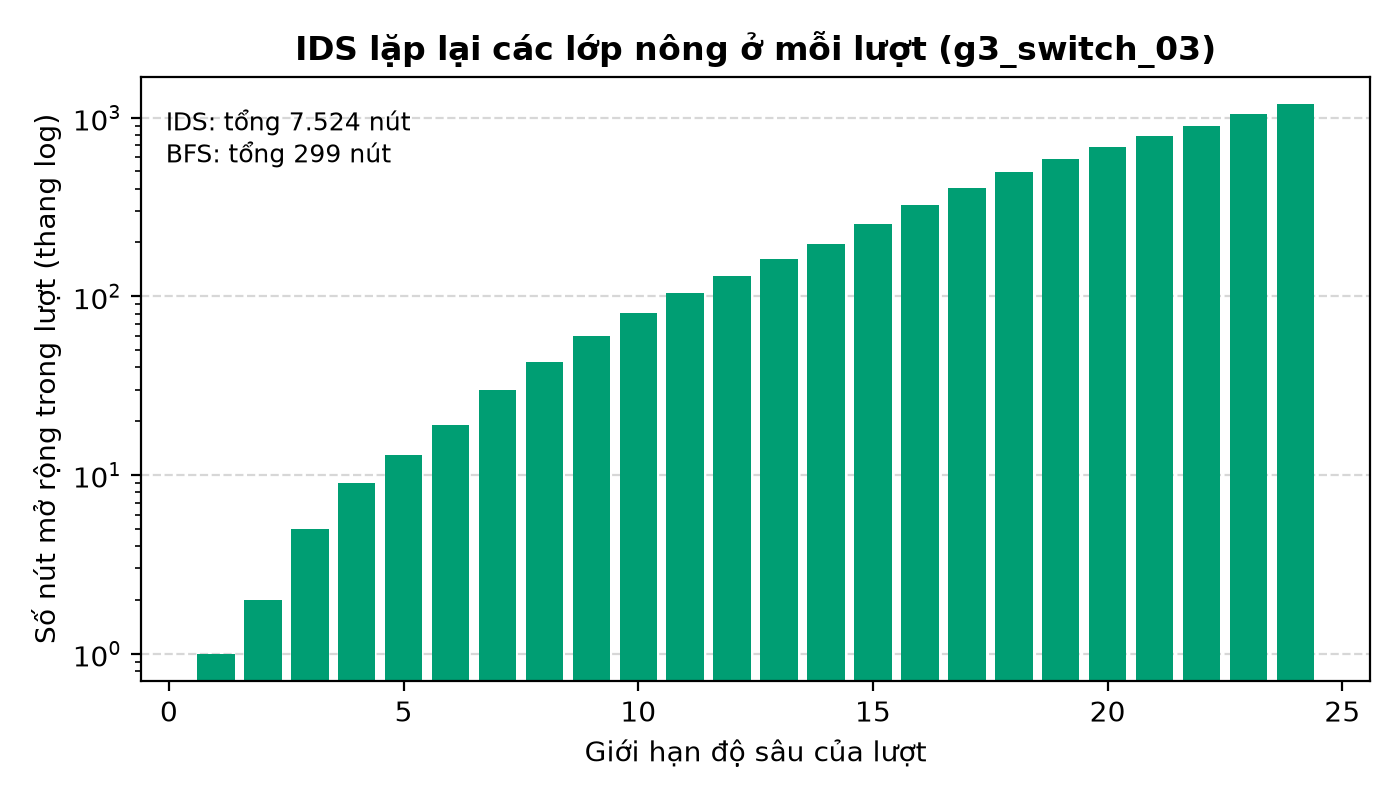
\includegraphics[width=\linewidth,height=0.45\textheight,keepaspectratio]{images/fig_ids_passes.png}
\caption{Số nút mở rộng ở từng lượt lặp của IDS trên màn g3\_switch\_03 (thang log): tổng 7.524 nút so với 299 nút của BFS. Chỉ riêng lượt cuối (giới hạn 24) đã mở rộng 1.189 nút, nhiều hơn toàn bộ BFS.}
\end{figure}

\subsubsection{Tính chất và chứng minh}

\textbf{Tính đầy đủ.} Nếu đích ở độ sâu d* (số nước đi ngắn nhất), đến lượt giới hạn d* thuật toán sẽ tìm thấy nó (chứng minh bên dưới). Nếu đích không đạt tới được, mọi lượt đều không có đích; khi giới hạn đủ lớn để không còn nút nào bị cắt, thuật toán kết luận không giải được.

\textbf{Tính tối ưu theo số nước đi.} Khẳng định: sau lượt giới hạn L, mọi trạng thái có khoảng cách ngắn nhất k ≤ L đều đã được đưa vào ngăn xếp ít nhất một lần với độ sâu đúng bằng k. Chứng minh bằng quy nạp theo k: s0 có độ sâu 0. Nếu s có khoảng cách k+1 ≤ L thì tồn tại nút cha p có khoảng cách k, được đưa vào với độ sâu k theo giả thiết và được lấy ra mở rộng với độ sâu k \textless{} L (vì k \textless{} L). Khi đó s được sinh ra với độ sâu k+1. Nó được đưa vào ngăn xếp trừ khi đã có \texttt{reached[s]} ≤ k+1; mà \texttt{reached[s]} không thể nhỏ hơn khoảng cách thực k+1, nên trong cả hai trường hợp s đã được đưa vào với độ sâu k+1. Hệ quả: lượt đầu tiên tìm thấy đích là lượt L = d*, và đường đi trả về dài d* nước. Nhờ điều kiện ``độ sâu nhỏ hơn thì cho vào lại'', phép chứng minh này không bị phá bởi thứ tự duyệt kiểu DFS.

\textbf{Độ phức tạp.} Các trạng thái ở độ sâu nhỏ bị mở rộng lại ở mọi lượt, nên tổng số nút mở rộng lớn hơn BFS. Với cây có hệ số nhánh b đều, hệ số chi phí xấp xỉ b/(b−1); với đồ thị trạng thái của Bloxorz, hệ số nhánh hiệu dụng nhỏ (số nút mỗi lượt chỉ tăng khoảng 1,1 đến 1,5 lần khi giới hạn tăng thêm 1, Hình 3) nên chi phí lặp lại lớn. Thêm vào đó, một lượt với giới hạn L còn mở rộng nhiều hơn số trạng thái cách s0 tối đa L nước, do một trạng thái có thể bị mở rộng lại mỗi khi được phát hiện ở độ sâu nhỏ hơn trong cùng lượt; vì vậy lượt cuối ở Hình 3 (1.189 nút) vượt tổng của BFS (299 nút). Về bộ nhớ, \texttt{reached} và \texttt{parent} giữ mọi trạng thái của một lượt, nên IDS \textbf{không} còn bộ nhớ tuyến tính như IDS dạng cây mà cùng bậc với BFS (đo được gấp 1,2 đến 1,6 lần BFS).

\subsection{So sánh lý thuyết ba thuật toán}

{\renewcommand{\arraystretch}{1.25}
\begin{longtable}{|>{\raggedright\arraybackslash}p{0.161\linewidth}|>{\raggedright\arraybackslash}p{0.194\linewidth}|>{\raggedright\arraybackslash}p{0.200\linewidth}|>{\raggedright\arraybackslash}p{0.305\linewidth}|}
\hline
\textbf{Tiêu chí} & \textbf{BFS} & \textbf{DFS} & \textbf{IDS} \\ \hline
\endhead
\hline
\endlastfoot
Frontier & Hàng đợi FIFO & Ngăn xếp LIFO & Ngăn xếp LIFO, giới hạn độ sâu tăng dần \\ \hline
Thời điểm kiểm tra đích & Khi sinh nút con & Khi lấy ra khỏi ngăn xếp & Khi lấy ra khỏi ngăn xếp \\ \hline
Đầy đủ & Có & Có (nhờ \texttt{visited}) & Có \\ \hline
Tối ưu theo số nước đi & Có & Không & Có \\ \hline
Tối ưu theo \texttt{physics\_\allowbreak{}cost} & Không đảm bảo & Không & Không đảm bảo \\ \hline
Thời gian & O(\textbar{}S\textbar{}), chặn bởi O(b$^{d}$) & O(\textbar{}S\textbar{}) & Lớn hơn BFS nhiều lần do mở rộng lại \\ \hline
Bộ nhớ & O(\textbar{}S\textbar{}) & O(số trạng thái đã sinh) & O(\textbar{}S\textbar{}) cho mỗi lượt \\ \hline
Phát hiện màn không giải được & Có (frontier cạn) & Có (ngăn xếp cạn) & Có (lượt không bị cắt); nếu hết \texttt{max\_\allowbreak{}depth} thì chưa kết luận \\
\end{longtable}
}
